\documentclass[11pt]{charter}

% El títulos de la memoria, se usa en la carátula y se puede usar el cualquier lugar del documento con el comando \ttitle
\titulo{Desarrollo de sensor de corriente} 

% Nombre del posgrado, se usa en la carátula y se puede usar el cualquier lugar del documento con el comando \degreename
\posgrado{Carrera de Especialización en Sistemas Embebidos} 
%\posgrado{Carrera de Especialización en Internet de las Cosas} 
%\posgrado{Carrera de Especialización en Intelegencia Artificial}
%\posgrado{Maestría en Sistemas Embebidos} 
%\posgrado{Maestría en Internet de las cosas}

% Tu nombre, se puede usar el cualquier lugar del documento con el comando \authorname
\autor{Ing. Santiago Esteva} 

% El nombre del director y co-director, se puede usar el cualquier lugar del documento con el comando \supname y \cosupname y \pertesupname y \pertecosupname
\director{Esp. Ing. Bucafusco Franco}
\pertenenciaDirector{FIUBA} 
% FIXME:NO IMPLEMENTADO EL CODIRECTOR ni su pertenencia
\codirector{} % si queda vacio no se deberíá incluir 
\pertenenciaCoDirector{}

% Nombre del cliente, quien va a aprobar los resultados del proyecto, se puede usar con el comando \clientename y \empclientename
\cliente{Cristian Muzzio}
\empresaCliente{Hitec S.R.L.}

% Nombre y pertenencia de los jurados, se pueden usar el cualquier lugar del documento con el comando \jurunoname, \jurdosname y \jurtresname y \perteunoname, \pertedosname y \pertetresname.
\juradoUno{Nombre y Apellido (1)}
\pertenenciaJurUno{pertenencia (1)} 
\juradoDos{Nombre y Apellido (2)}
\pertenenciaJurDos{pertenencia (2)}
\juradoTres{Nombre y Apellido (3)}
\pertenenciaJurTres{pertenencia (3)}
 
\fechaINICIO{23 de Octubre de 2020}		%Fecha de inicio de la cursada de GdP \fechaInicioName
\fechaFINALPlanificacion{18 de Diciembre de 2020} 	%Fecha de final de cursada de GdP
\fechaFINALTrabajo{19 de Octubre de 2021}		%Fecha de defensa pública del trabajo final


\begin{document}

\maketitle
\thispagestyle{empty}
\pagebreak


\thispagestyle{empty}
{\setlength{\parskip}{0pt}
\tableofcontents{}
}
\pagebreak


\section{Registros de cambios}
\label{sec:registro}


\begin{table}[ht]
\label{tab:registro}
\centering
\begin{tabularx}{\linewidth}{@{}|c|X|c|@{}}
\hline
\rowcolor[HTML]{C0C0C0} 
Revisión & \multicolumn{1}{c|}{\cellcolor[HTML]{C0C0C0}Detalles de los cambios realizados} & Fecha      \\ \hline
1.0      & Creación del documento                                          & 23/10/2020 \\ \hline
1.1      & Desarrollo hasta sección 6 inclusive                            & 05/11/2020 \\ \hline
1.2      & Correcciones e historias de usuario                            & 15/11/2020 \\ \hline
1.3      & Desarrollo hasta sección 11 inclusive						 & 22/11/2020  \\ \hline
1.4      & Correcciones y desarrollo final						 		& 27/11/2020  \\ \hline
\end{tabularx}
\end{table}

\pagebreak



\section{Acta de constitución del proyecto}
\label{sec:acta}

\begin{flushright}
Buenos Aires, \fechaInicioName
\end{flushright}

\vspace{2cm}

Por medio de la presente se acuerda con el Ing. \authorname\hspace{1px} que su Trabajo Final de la \degreename\hspace{1px} se titulará ``\ttitle'', consistirá esencialmente en el prototipo preliminar de un desarrollo de un sensor de corriente de tres fases capaz de medir, procesar e informar diversos parámetros necesarios para el mantenimiento predictivo en la industria, y tendrá un presupuesto preliminar estimado de 600 hs de trabajo y \textcolor{red}{\$XXX}, con fecha de inicio \fechaInicioName\hspace{1px} y fecha de presentación pública \fechaFinalName.

Se adjunta a esta acta la planificación inicial.

\vfill

% Esta parte se construye sola con la información que hayan cargado en el preámbulo del documento y no debe modificarla
\begin{table}[ht]
\centering
\begin{tabular}{ccc}
\begin{tabular}[c]{@{}c@{}}Ariel Lutenberg \\ Director posgrado FIUBA\end{tabular} & \hspace{2cm} & \begin{tabular}[c]{@{}c@{}}\clientename \\ \empclientename \end{tabular} \vspace{2.5cm} \\ 
\multicolumn{3}{c}{\begin{tabular}[c]{@{}c@{}} \supname \\ Director del Trabajo Final\end{tabular}} \vspace{2.5cm} \\
%\begin{tabular}[c]{@{}c@{}}\jurunoname \\ Jurado del Trabajo Final\end{tabular}     &  & \begin{tabular}[c]{@{}c@{}}\jurdosname\\ Jurado del Trabajo Final\end{tabular}  \vspace{2.5cm}  \\
%\multicolumn{3}{c}{\begin{tabular}[c]{@{}c@{}} \jurtresname\\ Jurado del Trabajo Final\end{tabular}} \vspace{.5cm}                                                                     
\end{tabular}
\end{table}




\section{Descripción técnica-conceptual del proyecto a realizar}
\label{sec:descripcion}

En la industria química existen procesos continuos de fabricación que deben ser controlados de forma permanente para asegurar una calidad constante entre lotes de un mismo producto. Sumado a los controles en tiempo de ejecución, existen técnicas de mantenimiento predictivo que permiten prever posibles fallas en los actuadores del proceso que implican paros de emergencia o tiempos muertos, que concluyen en pérdidas parciales o totales del lote.
Dado que en la mayoría de estos procesos se utilizan motores eléctricos como actuadores, se abre una gran posibilidad de desarrollar diversos tipos de sensores para aplicar mantenimiento predictivo. En la bibliografía se pueden encontrar diversos métodos relacionados a evaluar el desgaste de un motor mediante el análisis de su corriente de consumo. Es por ello que la empresa \empclientename necesita un sensor de corriente capaz de medir, procesar y comparar datos estadísticos en dominio del tiempo y frecuencia.

Actualmente la empresa presta un servicio de mantenimiento predictivo mediante la plataforma comercial \textit{teBox} de la firma Terative, con análisis y reportes de datos en la nube y se encuentra en la búsqueda de un sensor de corriente que se adecúe a su plataforma. El presente proyecto busca cubrir esta necesidad y propone desarrollar un sensor de corriente trifásico capaz de medir, procesar, almacenar y comunicar parámetros específicos a través de la plataforma \textit{teBox}.

En la figura \ref{fig:diagBloques} se presenta un diagrama en bloques del sensor que se propone desarrollar con el nombre comercial de teSensor-TC (\textit{Trifasic Current Sensor}) . Se observa la unidad central de procesamiento con sus periféricos, los circuitos necesarios para la adaptación de señales, alimentación y comunicación y los cuatro sensores externos.

\vspace{25px}

\begin{figure}[htpb]
\centering 
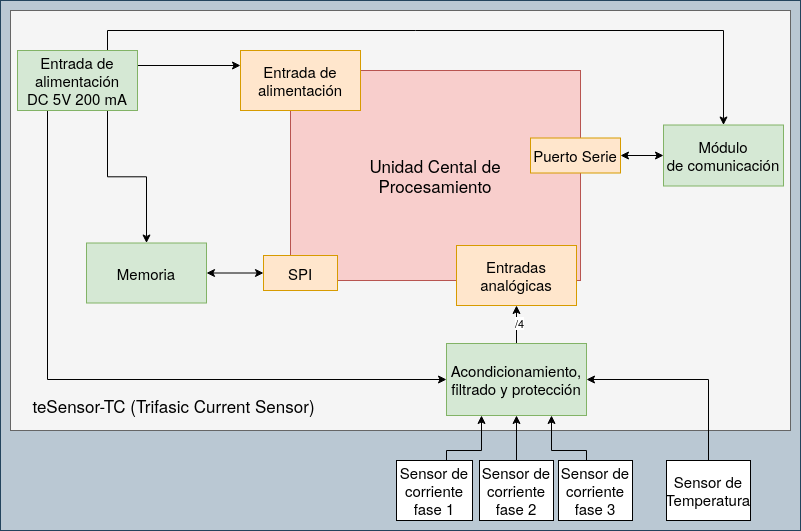
\includegraphics[width=.9\textwidth]{./Figuras/diagBloque.png}
\caption{Diagrama en bloques del sistema}
\label{fig:diagBloques}
\end{figure}

\vspace{25px}


El sensor debe medir los siguiente parámetros:
\begin{itemize}
\item Desplazamiento entre las tres fases
\item Valor estadístico (por fase) de corriente RMS AC 
\item Valor estadístico (por fase) de corriente DC
\item Valor estadístico (por fase) de factor de cresta
\item Valor pico de la corriente
\end{itemize}


Adicionalmente deberá procesar cada señal en frecuencia con la capacidad de extraer la frecuencia de máxima energía y energía de bandas predefinidas, contener una memoria externa para almacenar datos relacionados a valores de calibración de fábrica, valores de última calibración, máximos históricos de algunas variables de interés, fecha de cada dato almacenado, etc.

\section{Identificación y análisis de los interesados}
\label{sec:interesados}

\begin{table}[ht]
%\caption{Identificación de los interesados}
%\label{tab:interesados}
\begin{tabularx}{\linewidth}{@{}|l|X|X|l|@{}}
\hline
\rowcolor[HTML]{C0C0C0} 
Rol           & Nombre y Apellido & Organización 	& Puesto 	\\ \hline
Auspiciante y & \clientename      &\empclientename	&        	\\
Cliente		  &			   		  &					&        	\\ \hline
Responsable   & \authorname       & FIUBA        	& Alumno 	\\ \hline
Colaboradores & Martin Mello Teggia & FIUBA        	& Alumno 	\\ \hline
Orientador    & \supname	      & \pertesupname 	& Director	Trabajo final \\ \hline
Usuario final & Personal técnico del & \empclientename   	& Técnico       	\\ 
				& sector de instalaciones &              	&        	\\ \hline
\end{tabularx}
\end{table}
 
\begin{itemize}
\item Colaborador: Martín Mello Teggia, empleado de la empresa \empclientename  y estudiante de la especialización con gran experiencia en diseño de hardware y software.
\end{itemize}




\section{1. Propósito del proyecto}
\label{sec:proposito}

El propósito de este proyecto es desarrollar un sensor de corriente de tres fases capaz de medir, procesar e informar diversos parámetros necesarios para el mantenimiento predictivo en la industria química.

\section{2. Alcance del proyecto}
\label{sec:alcance}

El proyecto incluye los siguientes puntos:
\begin{itemize}
\item El diseño e implementación del hardware.
\item El desarrollo del firmware capaz de recolectar los datos, procesarlos y enviarlos mediante el protocolo de comunicación específico de \textit{teBox} en modelo maestro-esclavo.
\item Sensado de temperatura ambiental para conocer el modo de operación.
\item Desarrollo de una memoria técnica del proyecto.
\end{itemize}

El proyecto no incluye los siguientes puntos:
\begin{itemize}
\item El diseño y construcción de \textit{packaging} asociado para la distribución del producto.
\item El análisis de los datos recolectados y procesados.
\end{itemize}

\section{3. Supuestos del proyecto}
\label{sec:supuestos}

Para el desarrollo del presente proyecto se supone que:

\begin{itemize}
\item Todos los materiales necesarios para la implementación serán suministrados por \empclientename.
\item La importación de componentes no estará restringida y tomará un tiempo menor a 3 meses.
\item Se contará con asistencia por parte de \empclientename \space para el montaje de los componentes en el PCB.
\item \empclientename \space cuenta con todos los equipos para la medición y validación del prototipo.
\end{itemize}


\section{4. Requerimientos}
\label{sec:requerimientos}


A continuación se listan los requerimientos en prioridad descendente:

\begin{enumerate}
\item Grupo de requerimientos asociados al sistema
	\begin{enumerate}
	\item La alimentación por cable debe ser de 5 V con un consumo máximo de 200 mA. \label{req1}
	\item El sistema utilizará sensores disponibles comercialmente para la adquisición de la corriente y temperatura.
	\item El sistema deberá ser capaz de tomar muestras de los tres sensores de corriente en simultaneo al período de muestreo fijo.
	\item El sistema deberá poseer una memoria no volátil para registrar datos como valores máximos, parámetros de calibración, etc. 
	\item El sistema debe medir la temperatura ambiental de operación, rango de medición 0 - 50 centígrados.
	\item El sistema incorporará diseño y elementos que aseguren bajo consumo de energía (requerimiento 1.1).
	\item Los indicadores de situación serán enviados a la plataforma \textit{teBox}.
	\item El sistema deberá tomar muestras de los sensores externos con una tasa de muestreo de 1 kHz de frecuencia.
	\item El sistema deberá contar con una resolución de 16 bits (15 bits + signo).
	\end{enumerate}
\item Grupo de requerimientos asociados a la comunicación de datos
	\begin{enumerate}
	\item El protocolo de comunicación está definido por la plataforma \textit{teBox}.
	\item El sensor se comporta como esclavo y la plataforma \textit{teBox} como maestro.
	\end{enumerate}
\item Grupo de requerimientos asociados con el sensor de corriente
	\begin{enumerate}
	\item El sensor debe ser de efecto Hall.
	\item El sensor debe detectar corriente continua, alterna y de pulsos.
	\item El sensor debe ser de núcleo partido.
	\item El sensor debe ser de bajo consumo (máximo 20 mA).
	\end{enumerate}
\item Grupo de requerimientos asociados a testing
	\begin{enumerate}
	\item Se deberá testear cada módulo del hardware en forma individual y luego en conjunto.
	\item Se deberán validar los requerimientos detallados en el informe especificación de requerimientos de software CORRIENTE-ER-0001.
	\item Luego de la integración de hardware y software se deben realizar pruebas de funcionamiento. Lectura de dato sensado, almacenamiento en memoria, comunicación con plataforma, etc.
	\item Realizar la prueba integral del sistema en el caso de uso principal. 
	\end{enumerate}
\item Grupo de requerimientos asociados con la documentación
	\begin{enumerate}
	\item Se deberá generar una planificación completa del proyecto con los diferentes puntos a seguir durante el desarrollo del sensor.
	\item Se utilizarán informes de avance dirigidos al cliente y director con la finalidad de controlar los puntos planificados.
	\item Se deberá confeccionar una memoria técnica para el proyecto.
	\item Se deberá confeccionar un manual de uso en lenguaje  sencillo dirigido a un lector que podrá no contar con conocimiento técnico.
	\item Se deberá confeccionar un manual de instalación.
	\end{enumerate}
\end{enumerate}


\section{Historias de usuarios (\textit{Product backlog})}
\label{sec:backlog}

A continuación se detallan las historias de usuarios para el sistema con su respectiva puntuación. El criterio se toma de 1 (baja dificultad) - 4 (alta dificultad).
\begin{itemize}
\item Como usuario quiero que el sistema sea capaz de adquirir los datos de tres sensores de corriente con el objetivo de calcular el desgaste de un motor. (4)
\item Como cliente quiero que el sensado no sea invasivo ya que puede interferir en el proceso principal. (1)
\item Como usuario quiero recibir los datos en la plataforma con el objetivo de aplicar técnicas de mantenimiento preventivo. (2)
\item Como usuario quiero conocer la temperatura ambiente de trabajo del sensor para prevenir fallas por alta temperatura de operación. (1)
\item Como cliente quiero que el sistema sea capaz de comunicarse mediante el protocolo de \textit{teBox} con el objetivo de sumar un sensor a la plataforma. (4)
\item Como usuario quiero almacenar datos de interés en una memoria con el objetivo de independizar la adquisición de la comunicación. (3)
\item Como usuario quiero tener la capacidad de modificar parámetros de medición del sistema con el objetivo de calibrarlo. (2)
\end{itemize}

\section{5. Entregables principales del proyecto}
\label{sec:entregables}

\begin{itemize}
\item Prototipo funcional
\item Manual de uso
\item Diagrama esquemático electrónico del hardware
\item Código fuente
\item Manual de instalación
\item Informe final

\end{itemize}


\section{6. Desglose del trabajo en tareas}
\label{sec:wbs}

\begin{enumerate}
\item Análisis preliminar (48 hs)
	\begin{enumerate}
	\item Estudio sobre mantenimiento predictivo (10 hs)
	\item Investigación sobre posibles sensores de corriente (10 hs)
	\item Realizar el plan del proyecto (28 hs)
	\end{enumerate}
\item Hardware (140 hs)
	\begin{enumerate}
	\item Selección de componentes (12 hs)
	\item Diseño del circuito esquemático (28 hs)
	\item Diseño del PCB (30 hs)
	\item Fabricación y ensamblado del PCB (30 hs)
	\item Pruebas y validación del hardware (40 hs)
	\end{enumerate}
\item Firmware (154 hs)
	\begin{enumerate}
	\item Desarrollo de arquitectura del firmware  (16 hs)
	\item Diseño de firmware (32 hs)
	\item Análisis de riesgos de firmware (10 hs)
	\item Desarrollo de pruebas para firmware (32 hs)
	\item Programación del firmware (40 hs)
	\item Verificación y validación del firmware (24 hs)
	\end{enumerate}
\item Integración (157 hs)
	\begin{enumerate}
	\item Integración de los módulos constitutivos (32 hs)
	\item Pruebas de sensado (30 hs)
	\item Pruebas de almacenamiento de datos(30 hs)
	\item Pruebas de comunicación(30 hs)	
	\item Corrección de errores (35 hs)
	\end{enumerate}
\item Procesos finales (104 hs)
	\begin{enumerate}
	\item Elaboración del informe de avance (15 hs)
	\item Evaluación de requerimientos (25 hs)
	\item Elaboración de la memoria del proyecto (30 hs)
	\item Preparación de la presentación final (34 hs)
	\end{enumerate}
\end{enumerate}

Cantidad total de horas: 603 hs


\section{7. Diagrama de Activity On Node}
\label{sec:AoN}

En la Figura \ref{fig:AoN} se observa el diagrama de \textit{Activity on Node} con los tiempos en horas de trabajo. El camino critico señalado en negro tanto en las flechas como los recuadros de actividades da un total de 345 horas de trabajo.

\begin{figure}[htpb]
\centering 
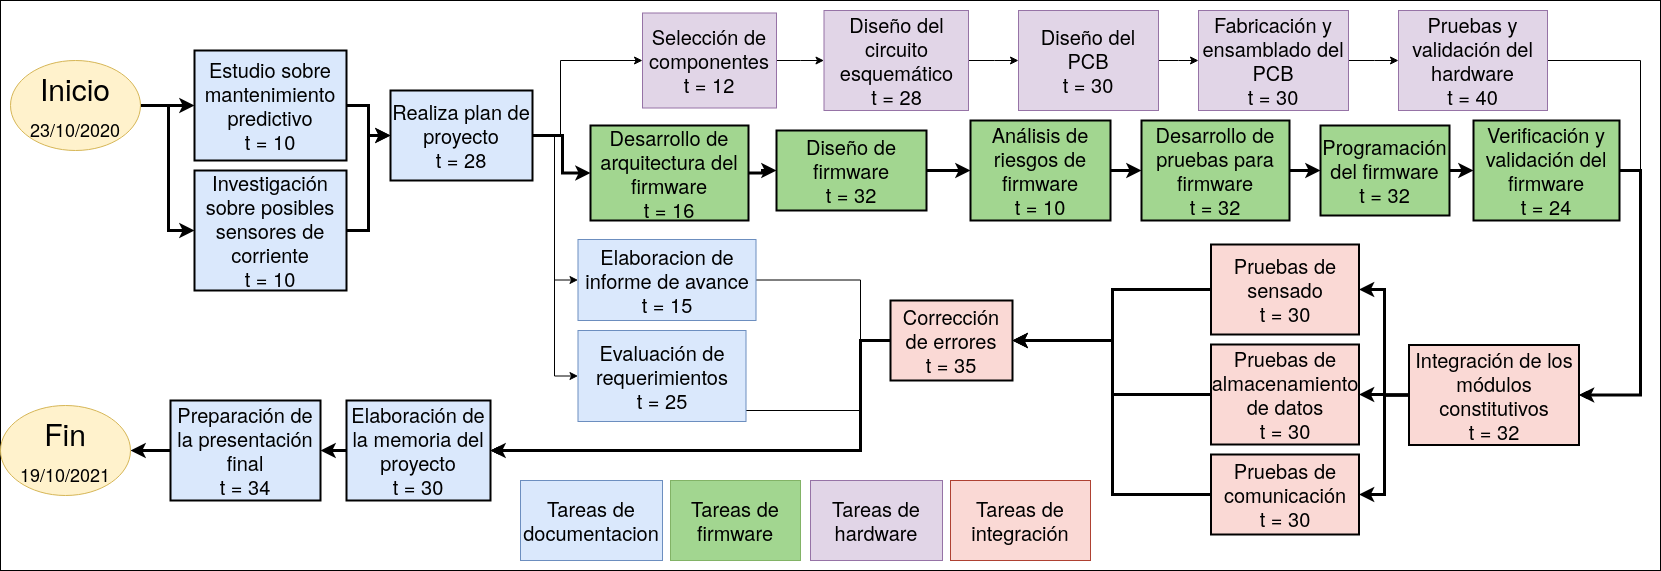
\includegraphics[width=1\textwidth]{./Figuras/AoN.png}
\caption{Diagrama en \textit{Activity on Node}}
\label{fig:AoN}
\end{figure}


\section{8. Diagrama de Gantt}
\label{sec:gantt}

En la figura \ref{fig:gantt} se muestra el diagrama de gantt correspondiente a las tareas detalladas en el cuadro. Se toma un calendario con 5 días laborales por semana y se estima un trabajo de veinte horas semanales dividido en cuatro horas diarias.

\begin{table}[htpb]
\centering
\begin{tabularx}{\linewidth}{@{}|c|X|c|c|c|c|@{}}
\hline
\rowcolor[HTML]{C0C0C0} 
Tarea & Nombre & Duración & Inicio & Final & Predecesor \\ \hline
1 & Análisis preliminar & 11 dias &  10/23/2020 & 10/30/2020 & \\ \hline
2 & Estudio sobre mantenimiento predictivo &  10 hs & 10/23/2020 & 	10/26/2020	 &\\ \hline
3 & Investigación sobre posibles sensores de corriente &  10 hs & 10/23/2020 & 10/26/2020	 & \\ \hline
4 & Realizar el plan del proyecto &  28 hs & 10/27/2020 & 	10/30/2020 & 2, 3 \\ \hline		
5 & Hardware &  45.4 días & 11/04/2020 & 	12/04/2020 & 1\\ \hline
6 & Selección de componentes &  12 hs & 11/04/2020 & 	11/05/2020 & 4\\ \hline
7 & Diseño del circuito esquemático &  28 hs & 11/06/2020 & 	11/11/2020	 &6\\ \hline
8 & Diseño del PCB &  30 hs & 11/16/2020 & 	11/19/2020 &7\\ \hline
9 & Fabricación y ensamblado del PCB &  30 hs & 11/24/2020 & 	11/27/2020	 & 8\\ \hline
10 & Pruebas y validación del hardware &  40 hs & 11/27/2020 & 	12/04/2020	 & 9	\\ \hline
11 & Firmware &  38.5 días &11/05/2020	 & 12/02/2020 &  1\\ \hline
12 & Desarrollo de arquitectura del firmware &   16 hs & 11/05/2020 & 	11/06/2020 & 4\\ \hline
13 & Diseño de firmware &  32 hs & 11/09/2020 & 	11/12/2020 & 12\\ \hline
14 & Análisis de riesgos de firmware &  10 hs & 11/13/2020 & 	11/16/2020 & 13\\ \hline
15 & Desarrollo de pruebas para firmware &  32 hs & 11/16/2020 & 	11/20/2020 & 14\\ \hline
16 & Programación del firmware &  40 hs & 11/20/2020 & 	11/27/2020 & 15\\ \hline
17 & Verificación y validación del firmware  & 24 hs &11/27/2020 & 	12/02/2020 & 16 \\ \hline
18 & Integración &  24.25 dias & 12/04/2020 & 	12/22/2020 &5, 11\\ \hline
19 & Integración de los módulos constitutivos &  32 hs & 12/04/2020 & 	12/10/2020 & 10, 17\\ \hline
20 & Pruebas de sensado &  30 hs & 12/10/2020 & 	12/16/2020 & 19\\ \hline
21 & Pruebas de almacenamiento de datos & 30 hs & 12/10/2020 & 	12/16/2020 &19\\ \hline
22 & Pruebas de comunicación & 30 hs & 12/10/2020 & 	12/16/2020 & 19\\ \hline
23 & Corrección de errores &  35 hs & 12/16/2020 & 	12/22/2020 &20, 21, 22\\ \hline
24 & Procesos finales &  77.75 días & 11/10/2020 & 	01/01/2021 & \\ \hline
25 & Elaboración del informe de avance &  15 hs & 11/10/2020 & 	11/11/2020 & 4\\ \hline
26 & Evaluación de requerimientos &  25 hs & 11/11/2020 & 	11/16/2020 & 4\\ \hline
27 & Elaboración de la memoria del proyecto &  30 hs & 12/22/2020 & 	12/28/2020 & 23, 25, 26\\ \hline
28 & Preparación de la presentación final &  34 hs &12/28/2020 & 	01/01/2021 &  27\\ 
\hline
\end{tabularx}%
\label{tab:gantt}
\end{table}

\begin{figure}[htpb]
\begin{subfigure}[b]{1\textwidth}
\centering 
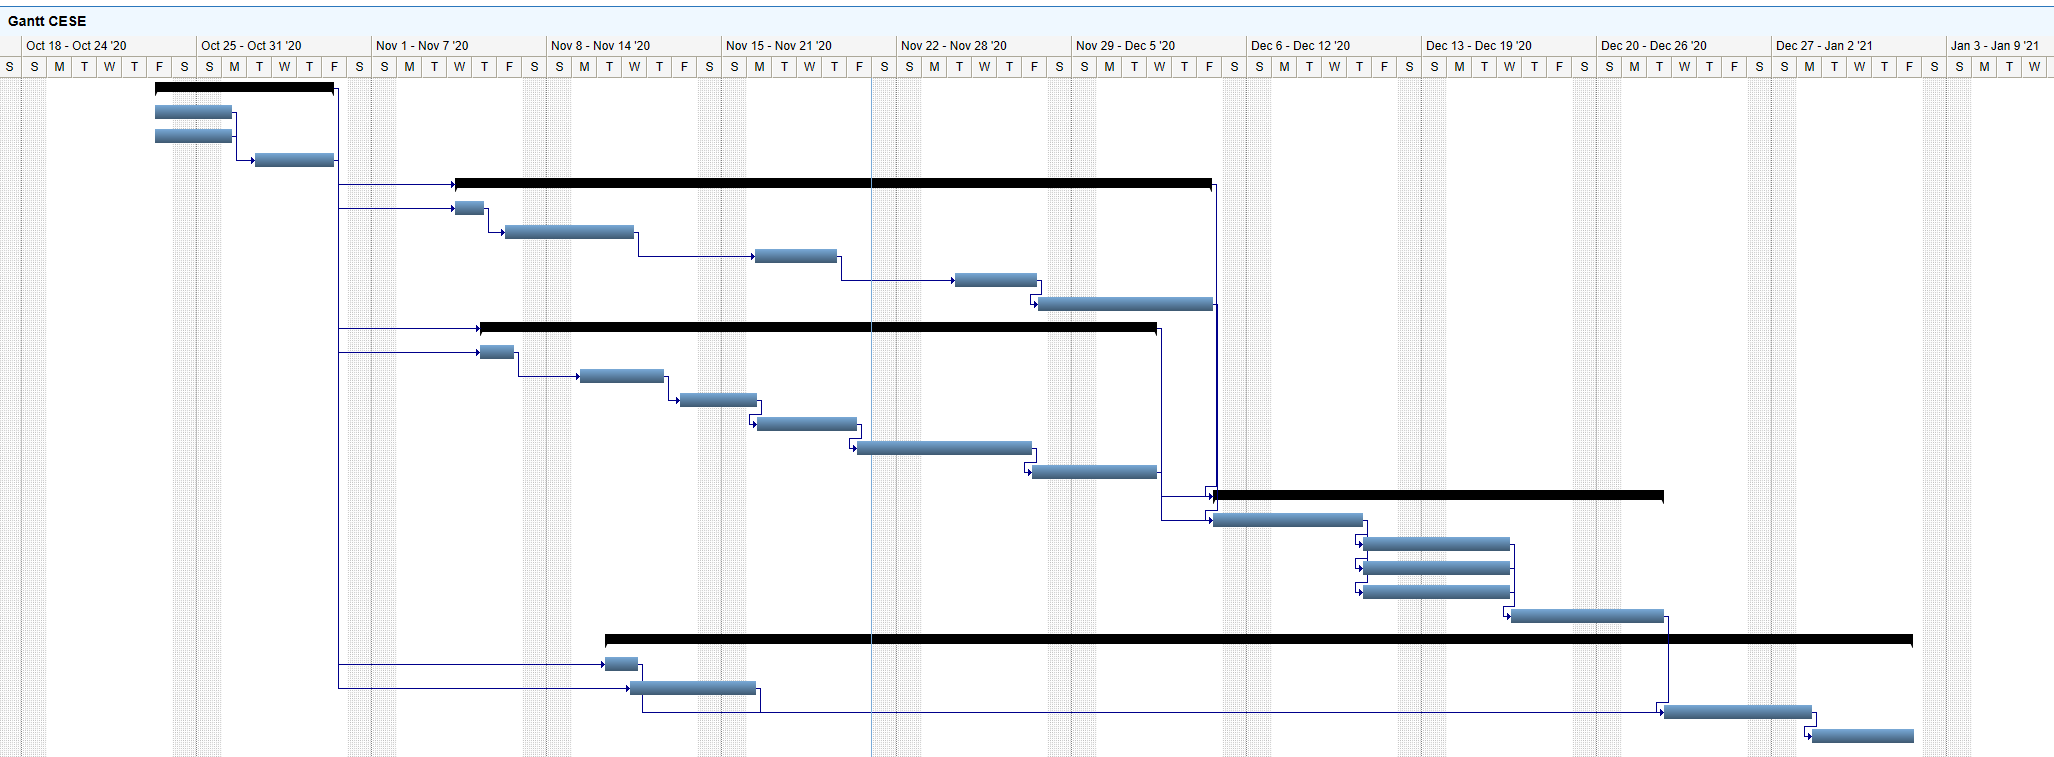
\includegraphics[width=.93\textwidth]{./Figuras/gant.png}
\end{subfigure}
\begin{subfigure}[b]{1\textwidth}
\centering 
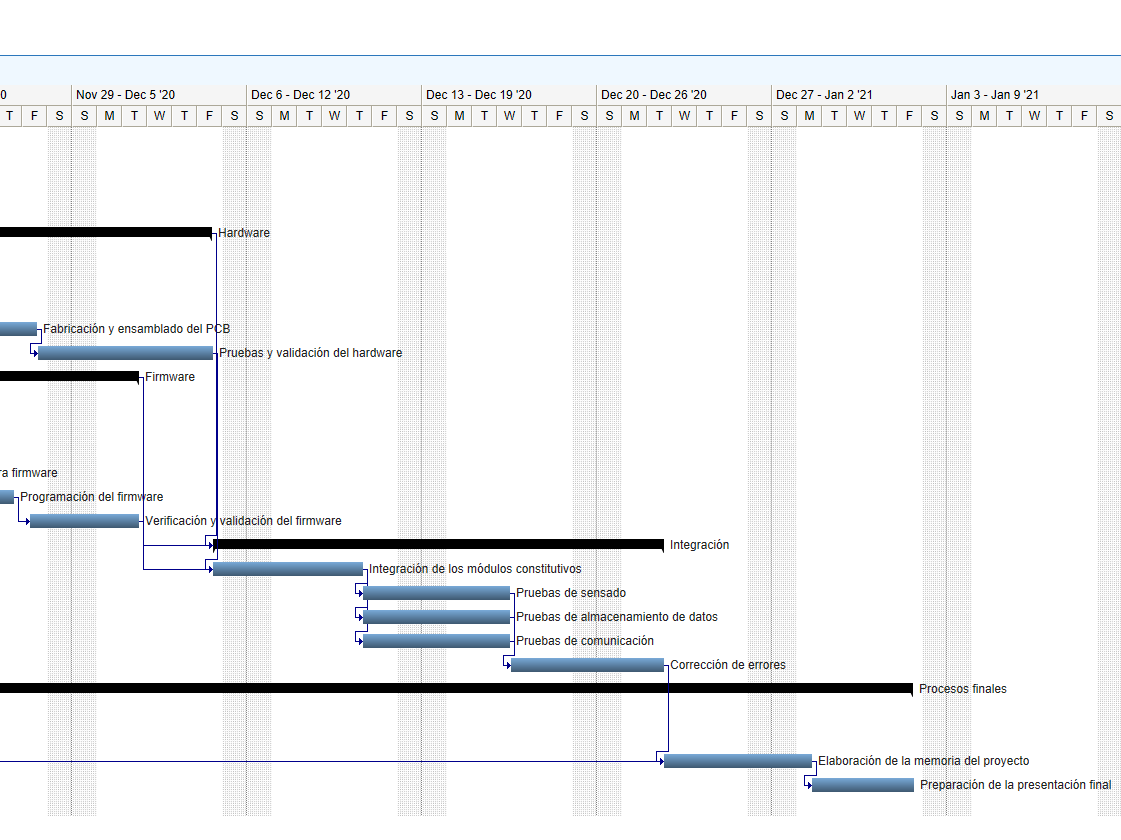
\includegraphics[width=.93\textwidth]{./Figuras/gant2.png}
\end{subfigure}
\caption{Diagrama de gantt}
\label{fig:gantt}
\end{figure}

\section{9. Matriz de uso de recursos de materiales}
\label{sec:recursos}

\begin{table}[H]
\label{tab:recursos1}
\centering
\begin{tabularx}{\linewidth}{@{}|c|X|c|c|c|c|@{}}
\hline
\cellcolor[HTML]{C0C0C0} & \cellcolor[HTML]{C0C0C0} & \multicolumn{4}{c|}{\cellcolor[HTML]{C0C0C0}Recursos requeridos (horas)} \\ \cline{3-6} 
\multirow{-2}{*}{\cellcolor[HTML]{C0C0C0}\begin{tabular}[c]{@{}c@{}}Código\\ WBS\end{tabular}} & \multirow{-2}{*}{\cellcolor[HTML]{C0C0C0}\begin{tabular}[c]{@{}c@{}}Nombre \\ tarea\end{tabular}} & Computadora & Soldador & Laboratorio & Prototipo \\ \hline
1.1 & Estudio sobre mantenimiento predictivo& 10 &  &  &  \\ \hline
1.2 & Investigación sobre posibles sensores de corriente& 10 &  &  &  \\ \hline
1.3 & Realizar el plan del proyecto& 28 &  &  &  \\ \hline
2.1 & Selección de componentes& 12 &  &  &  \\ \hline
2.2 & Diseño del circuito esquemático& 28 &  &  &  \\ \hline
2.3 & Diseño del PCB & 30 &  &  &  \\ \hline
2.4 & Fabricación y ensamblado del PCB &  & 30 &  &  \\ \hline
2.5 & Pruebas y validación del hardware &  &  & 40 &  \\ \hline
3.1 & Desarrollo de arquitectura del firmware  & 16 &  &  &  \\ \hline
3.2 & Diseño de firmware & 32 &  &  &  \\ \hline
3.3 & Análisis de riesgos de firmware & 10 &  &  &  \\ \hline
3.4 & Desarrollo de pruebas para firmware & 32 &  &  &  \\ \hline
3.5 & Programación del firmware &  &  &  & 40 \\ \hline
3.6 & Verificación y validación del firmware &  &  &  & 24 \\ \hline
4.1 & Integración de los módulos constitutivos &  &  &  & 32 \\ \hline
4.2 & Pruebas de sensado &  &  & 20 & 10 \\ \hline
4.3 & Pruebas de almacenamiento de datos&  &  &  & 30 \\ \hline
4.4 & Pruebas de comunicación &  &  &  & 30 \\ \hline
4.5 & Corrección de errores & 10 &  & 10 & 10 \\ \hline
5.1 & Elaboración del informe de avance& 15 &  &  &  \\ \hline
5.2 & Evaluación de requerimientos & 25 &  &  &  \\ \hline
5.3 & Elaboración de la memoria del proyecto & 30 &  &  &  \\ \hline
5.4 & Preparación de la presentación final & 34 &  &  &  \\ \hline
\end{tabularx}
\end{table}

\newpage
\section{10. Presupuesto detallado del proyecto}
\label{sec:presupuesto}

\begin{table}[htpb]
\centering
\begin{tabularx}{\linewidth}{@{}|X|c|r|r|@{}}
\hline
\rowcolor[HTML]{C0C0C0} 
\multicolumn{4}{|c|}{\cellcolor[HTML]{C0C0C0}COSTOS DIRECTOS} \\ \hline
\rowcolor[HTML]{C0C0C0} 
Descripción &
  \multicolumn{1}{c|}{\cellcolor[HTML]{C0C0C0}Cantidad} &
  \multicolumn{1}{c|}{\cellcolor[HTML]{C0C0C0}Valor unitario} &
  \multicolumn{1}{c|}{\cellcolor[HTML]{C0C0C0}Valor total} \\ \hline
 Salario ingeniero junior&
  \multicolumn{1}{c|}{573} &
  \multicolumn{1}{c|}{\$ 475} &
  \multicolumn{1}{c|}{\$ 272.175} \\ \hline
 Salario técnico &
  \multicolumn{1}{c|}{30} &
  \multicolumn{1}{c|}{\$ 250} &
  \multicolumn{1}{c|}{\$ 7.500} \\ \hline
\multicolumn{1}{|l|}{Materiales del prototipo} &
   \multicolumn{1}{c|}{2}&
   \multicolumn{1}{c|}{\$ 10.000}&
   \multicolumn{1}{c|}{\$ 20.000}\\ \hline
\multicolumn{1}{|l|}{Fabricación de PCB} &
   \multicolumn{1}{c|}{2}&
   \multicolumn{1}{c|}{\$ 2.000}&
   \multicolumn{1}{c|}{\$ 4.000}\\ \hline
\multicolumn{3}{|c|}{SUBTOTAL} &
  \multicolumn{1}{c|}{\$ 303.675} \\ \hline
\rowcolor[HTML]{C0C0C0} 
\multicolumn{4}{|c|}{\cellcolor[HTML]{C0C0C0}COSTOS INDIRECTOS} \\ \hline
\rowcolor[HTML]{C0C0C0} 
Descripción &
  \multicolumn{1}{c|}{\cellcolor[HTML]{C0C0C0}Cantidad} &
  \multicolumn{1}{c|}{\cellcolor[HTML]{C0C0C0}Valor unitario} &
  \multicolumn{1}{c|}{\cellcolor[HTML]{C0C0C0}Valor total} \\ \hline
\multicolumn{1}{|l|}{45 \% del costo directo} &
   \multicolumn{1}{c|}{1}&
   \multicolumn{1}{c|}{\$ 136.600}&
   \multicolumn{1}{c|}{\$ 136.600} \\ \hline
\multicolumn{1}{|l|}{Impuestos materiales 10 \%} &
   \multicolumn{1}{c|}{1}&
   \multicolumn{1}{c|}{\$ 1200}&
   \multicolumn{1}{c|}{\$ 1200} \\ \hline
\multicolumn{1}{|l|}{Envio material y PCB} &
   \multicolumn{1}{c|}{1}&
   \multicolumn{1}{c|}{\$ 5000}&
   \multicolumn{1}{c|}{\$ 5000} \\ \hline
\multicolumn{3}{|c|}{SUBTOTAL} &
  \multicolumn{1}{c|}{\$ 142.800} \\ \hline
\rowcolor[HTML]{C0C0C0}
\multicolumn{3}{|c|}{TOTAL} &
 \multicolumn{1}{c|}{\$ 446.475}  \\ \hline
\end{tabularx}%
\end{table}


\section{11. Matriz de asignación de responsabilidades}
\label{sec:responsabilidades}

En la siguiente tabla se asignan las responsabilidades y el manejo de la autoridad.

\begin{table}[htpb]
\centering
\resizebox{\textwidth}{!}{%
\begin{tabular}{|c|c|c|c|c|c|}
\hline
\rowcolor[HTML]{C0C0C0} 
\cellcolor[HTML]{C0C0C0} &
  \cellcolor[HTML]{C0C0C0} &
  \multicolumn{4}{|c|}{\cellcolor[HTML]{C0C0C0}Listar todos los nombres y roles del proyecto} \\ \cline{3-6} 
\rowcolor[HTML]{C0C0C0} 
\cellcolor[HTML]{C0C0C0} &
  \cellcolor[HTML]{C0C0C0} &
  Responsable &
  Orientador &
  Equipo &
  Cliente \\ \cline{3-6} 
\rowcolor[HTML]{C0C0C0} 
\multirow{-3}{*}{\cellcolor[HTML]{C0C0C0}\begin{tabular}[c]{@{}c@{}}Código\\ WBS\end{tabular}} &
  \multirow{-3}{*}{\cellcolor[HTML]{C0C0C0}Nombre de la tarea} &
  \authorname &
  \supname &
  Martín Mello Teggia &
  \clientename \\ \hline
1.1 & Estudio sobre mantenimiento predictivo& S & I & P & C \\ \hline
1.2 & Investigación sobre posibles sensores de corriente& P & I & S & C \\ \hline
1.3 & Realizar el plan del proyecto& P & I & C & A \\ \hline
2.1 & Selección de componentes& P & C & S & A \\ \hline
2.2 & Diseño del circuito esquemático& P & I & C & A \\ \hline
2.3 & Diseño del PCB & P & I & C & A \\ \hline
2.4 & Fabricación y ensamblado del PCB & P & I & S & A \\ \hline
2.5 & Pruebas y validación del hardware & P & I & C & I \\ \hline
3.1 & Desarrollo de arquitectura del firmware  & P & C & I & C \\ \hline
3.2 & Diseño de firmware & P & I & C & A \\ \hline
3.3 & Análisis de riesgos de firmware & P & I & C & I \\ \hline
3.4 & Desarrollo de pruebas para firmware & P & I & C & A \\ \hline
3.5 & Programación del firmware & P & I & C & I \\ \hline
3.6 & Verificación y validación del firmware & P & C & S & A \\ \hline
4.1 & Integración de los módulos constitutivos & P & I & S & I \\ \hline
4.2 & Pruebas de sensado & P & I & S & A \\ \hline
4.3 & Pruebas de almacenamiento de datos& P & I & S & A \\ \hline
4.4 & Pruebas de comunicación & P & I & S & A \\ \hline
4.5 & Corrección de errores & P & C & S & I \\ \hline
5.1 & Elaboración del informe de avance& P & A & I & I \\ \hline
5.2 & Evaluación de requerimientos & P & C & I & A \\ \hline
5.3 & Elaboración de la memoria del proyecto & P & A & I & I \\ \hline
5.4 & Preparación de la presentación final & P & A & I & I \\ \hline\end{tabular}%
}
\end{table}

{\footnotesize
Referencias:
\begin{itemize}
	\item P = Responsabilidad Primaria
	\item S = Responsabilidad Secundaria
	\item A = Aprobación
	\item I = Informado
	\item C = Consultado
\end{itemize}
} %footnotesize


\section{12. Gestión de riesgos}
\label{sec:riesgos}

 
Riesgo 1: Daños en el prototipo
\begin{itemize}
\item Severidad (S): 10.\\
El daño del prototipo puede darse a partir de la integración en cualquiera de las siguiente etapas lo cual conlleva a una perdida de tiempo y recursos para arreglarlo o en el peor de los casos producir otro prototipo.
\item Probabilidad de ocurrencia (O): 4.\\
El personal que manipula el prototipo tiene experiencia y capacidad para ello. 
\end{itemize}   

Riesgo 2: Firmware inadecuado
\begin{itemize}
\item Severidad (S): 7.\\
La planificación, elección e implementación errónea del firmware que no cubra los requerimientos iniciales genera una perdida de tiempo.
\item Probabilidad de ocurrencia (O): 6.\\
Poca experiencia en desarrollos de firmware similares. 
\end{itemize}

Riesgo 3: Pérdida total o parcial del código desarrollado
\begin{itemize}
\item Severidad (S): 9.\\
Implicaría importantes retrasos en el desarrollo del trabajo dificultando el cumplimiento con la fecha de entrega.
\item Probabilidad de ocurrencia (O): 1.\\
Se utilizará durante toda la fase de desarrollo un sistema de control de versiones y \textit{backup} en la nube.
\end{itemize}

Riesgo 4: Retardos en la entrega de materiales
\begin{itemize}
\item Severidad (S): 4.\\
Genera retardo en los plazos de entrega del proyecto.
\item Probabilidad de ocurrencia (O): 2.\\
Con la planificación previa se planifica los materiales a utilizar y se realiza la compra con antelación. 
\end{itemize}

Riesgo 5: Errores en el diseño del hardware 
\begin{itemize}
\item Severidad (S): 5.\\
Presenta perdidas de tiempo y mayores gastos en la necesidad de un nuevo diseño.
\item Probabilidad de ocurrencia (O): 3.\\
El diseño de cada etapa se analiza y deben ser aprobados previo a la construcción. 
\end{itemize}

b) Tabla de gestión de riesgos:  

\begin{table}[H]
\centering
\begin{tabularx}{\linewidth}{@{}|X|c|c|c|c|c|c|@{}}
\hline
\rowcolor[HTML]{C0C0C0} 
Riesgo & S & O & RPN & S* & O* & RPN* \\ \hline
Daños en el prototipo	& 10  & 4  &   40  &  8  &  2  &  16    \\ \hline
Firmware inadecuado	& 9  & 6  &   54  &  7  &  2  &   14   \\ \hline
Pérdida total o parcial del código desarrollado	& 8  & 2  &   16  &    &    &      \\ \hline
Retardos en la entrega de materiales	&  4 & 3  &  12   &    &    &      \\ \hline
Errores en el diseño del hardware	& 5  & 3  &   15  &    &    &      \\ \hline
\end{tabularx}%
\end{table}

Criterio adoptado: 
Se tomarán medidas de mitigación en los riesgos cuyos números de RPN sean mayores a 25.

Nota: los valores marcados con (*) en la tabla corresponden luego de haber aplicado la mitigación.

c) Plan de mitigación de los riesgos que originalmente excedían el RPN máximo establecido:
 
Riesgo 1: Se genera un protocolo para manipular el prototipo con todos los cuidados y dentro del proyecto se cotizan 2 prototipos funcionales.
\begin{itemize}
\item Severidad (S): 8.\\
Sigue siendo severo pero al tener dos prototipos, el daño de uno de ellos baja este número.
\item Probabilidad de ocurrencia (O): 2.\\
Al agregar la planificación baja un punto la probabilidad. 
\end{itemize}

Riesgo 2: Se capacita al personal.
\begin{itemize}
\item Severidad (S): 7.\\
Baja un punto pero sigue siendo alto ya que si ocurre representa una perdida de tiempo sumado a los gastos generados por las capacitaciones.
\item Probabilidad de ocurrencia (O): 2.\\
Luego de la capacitación se baja de forma considerable esta probabilidad. 
\end{itemize}


\section{13. Gestión de la calidad}
\label{sec:calidad}


\begin{enumerate}
\item Grupo de requerimientos asociados al sistema
	\begin{enumerate}
	\item La alimentación por cable debe ser de 5 V con un consumo máximo de 200 mA. \label{req1}
		\begin{itemize}
			\item Verificación: comprobar las hojas de datos de todos los componentes.  
			\item Validación: se medirá el consumo total del prototipo.  
		\end{itemize}
	\item El sistema utilizará sensores disponibles comercialmente para la adquisición de la corriente y temperatura.
		\begin{itemize}
			\item Verificación: 
			\item Validación: 
		\end{itemize}
	\item El sistema deberá ser capaz de tomar muestras de los tres sensores de corriente en simultaneo al período de muestreo fijo.
		\begin{itemize}
			\item Verificación: se verifica el código diseñado 
			\item Validación: se deberá realizar las pruebas de laboratorio con los tres sensores conectados y el análisis de los datos registrados
		\end{itemize}
	\item El sistema deberá poseer una memoria no volátil para registrar datos como valores máximos, parámetros de calibración, etc. 
		\begin{itemize}
			\item Verificación: análisis de hojas de datos
			\item Validación: prueba de escritura y lectura de datos
		\end{itemize}
	\item El sistema debe medir la temperatura ambiental de operación, rango de medición 0 - 50 centígrados.
		\begin{itemize}
			\item Verificación: consultar las hojas de datos de sensores de temperatura que cubran el rango necesario
			\item Validación: se realiza una prueba de laboratorio para varias temperaturas
		\end{itemize}
	\item El sistema incorporará diseño y elementos que aseguren bajo consumo de energía (requerimiento 1.1).
		\begin{itemize}
			\item Verificación: corroborar en la hoja de datos 
			\item Validación: medir el consumo en laboratorio de cada componente del hardware
		\end{itemize}
	\item Los indicadores de situación serán enviados a la plataforma \textit{teBox}.
		\begin{itemize}
			\item Verificación: se revisa el software
			\item Validación: se hará una prueba de laboratorio 
		\end{itemize}
	\item El sistema deberá tomar muestras de los sensores externos con una tasa de muestreo de 1 kHz de frecuencia.
		\begin{itemize}
			\item Verificación: control del modulo de entradas y el ADC del microcontrolador
			\item Validación: Primero se realizan pruebas del módulo hardware y luego se controla con el software los valores de lectura para varios puntos dentro del espectro 
		\end{itemize}
	\item El sistema deberá contar con una resolución de 16 bits (15 bits + signo).
		\begin{itemize}
			\item Verificación: lectura de hoja de datos del microcontrolador seleccionado
			\item Validación: pruebas de resolucion para el ADC 
		\end{itemize}
	\end{enumerate}
\item Grupo de requerimientos asociados a la comunicación de datos
	\begin{enumerate}
	\item El protocolo de comunicación está definido por la plataforma \textit{teBox}.
		\begin{itemize}
			\item Verificación: se revisa el protocolo en la etapa de diseño del software
			\item Validación: pruebas de comunicación con el prototipo.
		\end{itemize}
	\item El sensor se comporta como esclavo y la plataforma \textit{teBox} como maestro.
		\begin{itemize}
			\item Verificación: revisar el código de comunicación desarrollado 
			\item Validación: pruebas de comunicación con el prototipo y la plataforma 
		\end{itemize}
	\end{enumerate}
\item Grupo de requerimientos asociados con el sensor de corriente
	\begin{enumerate}
	\item El sensor debe ser de efecto Hall.
		\begin{itemize}
			\item Verificación: control de la hoja de datos del sensor
			\item Validación: prueba del sensor en el laboratorio
		\end{itemize}
	\item El sensor debe detectar corriente continua, alterna y de pulsos.
		\begin{itemize}
			\item Verificación: consulta con la hoja de datos y personal experto en el área
			\item Validación: prueba de laboratorio para los tres casos de corriente 
		\end{itemize}
	\item El sensor debe ser de núcleo partido.
		\begin{itemize}
			\item Verificación: consulta en hoja de datos
			\item Validación: comprobar el diseño al adquirirlo 
		\end{itemize}
	\item El sensor debe ser de bajo consumo (máximo 20 mA).
		\begin{itemize}
			\item Verificación: consulta en la hoja de datos
			\item Validación: prueba de consumo máximo en laboratorio 
		\end{itemize}
	\end{enumerate}
\item Grupo de requerimientos asociados a testing
	\begin{enumerate}
	\item Se deberá testear cada módulo del hardware en forma individual y luego en conjunto.
		\begin{itemize}
			\item Verificación: planificación en conjunto con el cliente de las pruebas 
			\item Validación: probar en laboratorio con el orden predeterminado
		\end{itemize}
	\item Se deberán validar los requerimientos detallados en el informe especificación de requerimientos de software CORRIENTE-ER-0001.
		\begin{itemize}
			\item Verificación: informe
			\item Validación: validación de los requerimientos detallados en el informe 
		\end{itemize}
	\item Luego de la integración de hardware y software se deben realizar pruebas de funcionamiento. Lectura de dato sensado, almacenamiento en memoria, comunicación con plataforma, etc.
		\begin{itemize}
			\item Verificación: planificar las pruebas a realizar en conjunto con el cliente 
			\item Validación: pruebas de laboratorio y de campo 
		\end{itemize}
	\item Realizar la prueba integral del sistema en el caso de uso principal. 
		\begin{itemize}
			\item Verificación: definir las pruebas
			\item Validación: pruebas iniciales en laboratorio y luego en campo 
		\end{itemize}
	\end{enumerate}
\item Grupo de requerimientos asociados con la documentación
	\begin{enumerate}
	\item Se deberá generar una planificación completa del proyecto con los diferentes puntos a seguir durante el desarrollo del sensor.
		\begin{itemize}
			\item Verificación: consultar con director y docentes de la maestría 
			\item Validación: aprobación por parte del director
		\end{itemize}
	\item Se utilizarán informes de avance dirigidos al cliente y director con la finalidad de controlar los puntos planificados.
		\begin{itemize}
			\item Verificación: consulta al cliente y director los períodos de avance 
			\item Validación: aprobación de cliente y director
		\end{itemize}
	\item Se deberá confeccionar una memoria técnica para el proyecto.
		\begin{itemize}
			\item Verificación: consulta a los docentes de la maestría y director
			\item Validación: corrección por parte de los docentes de la maestría
		\end{itemize}
	\item Se deberá confeccionar un manual de uso en lenguaje  sencillo dirigido a un lector que podrá no contar con conocimiento técnico.
		\begin{itemize}
			\item Verificación: consulta con personal técnico del cliente
			\item Validación: corrección por parte del cliente
		\end{itemize}
	\item Se deberá confeccionar un manual de instalación.
		\begin{itemize}
			\item Verificación: consulta con personal técnico del cliente
			\item Validación: corrección por parte del cliente
		\end{itemize}
	\end{enumerate}
\end{enumerate}


\section{14. Comunicación del proyecto}
\label{sec:comunicaciones}

El plan de comunicación del proyecto es el siguiente:

\begin{table}[htpb]
\centering
\begin{tabularx}{\linewidth}{@{}|X|C{2.4cm}|C{3cm}|C{1.8cm}|C{2cm}|C{2.1cm}|@{}}
\hline
\rowcolor[HTML]{C0C0C0} 
\multicolumn{6}{|c|}{\cellcolor[HTML]{C0C0C0}PLAN DE COMUNICACIÓN DEL PROYECTO}           \\ \hline
\rowcolor[HTML]{C0C0C0} 
¿Qué comunicar? & Audiencia & Propósito & Frecuencia & Método de comunicac. & Responsable \\ \hline
Definición de objetivos y alcances  &   \clientename , \supname        &    Evaluación    &     al inicio       &       email, reuniones               &     \authorname        \\ \hline
Notificación de avances                &    \clientename , \supname       &  Tener informado a los involucrados &      semanal      &           email, reuniones           &      \authorname       \\ \hline
Consultas técnicas                &      \clientename , \supname     & consultas para solucionar inconveniente&     semanal       &           email, reuniones           &      \authorname       \\ \hline
Resultados de pruebas                &     \clientename , \supname      & informar los resultados &     mensual       &         email, reuniones             &       \authorname      \\ \hline
Finalización y cierre                &    \supname       & Planificar la presentación del proyecto &     fin       &          email, reuniones            &        \authorname     \\ \hline
\end{tabularx}
\end{table}

\section{15. Gestión de compras}
\label{sec:compras}

La compra de componentes corre por parte del cliente.

\section{16. Seguimiento y control}
\label{sec:seguimiento}

\begin{longtable}{|m{1cm}|m{3.5cm}|m{2.2cm}|m{2cm}|m{3cm}|m{1.5cm}|}
\hline
\rowcolor[HTML]{C0C0C0} 
\multicolumn{6}{|c|}{\cellcolor[HTML]{C0C0C0}SEGUIMIENTO DE AVANCE}                                                                       \\ \hline
\rowcolor[HTML]{C0C0C0} 
Tarea del WBS 			& Indicador de avance & Frecuencia de reporte & Resp. de seguimiento & Persona a ser informada & Método de comunic. \\ \hline
\endfirsthead

\hline
\rowcolor[HTML]{C0C0C0} 
\multicolumn{6}{c}{\cellcolor[HTML]{C0C0C0}SEGUIMIENTO DE AVANCE}                                                                       \\ \hline
\rowcolor[HTML]{C0C0C0} 
Tarea del WBS 			& Indicador de avance & Frecuencia de reporte & Resp. de seguimiento & Persona a ser informada & Método de comunic. \\ \hline
\endhead

\multicolumn{6}{c}{Continúa}
\endfoot

\endlastfoot

1.1	& Fecha de inicio  & Única vez al comienzo & \authorname & \clientename, \supname & email \\ \hline
2.1	& Avance de las subtareas  & Mensual mientras dure la tarea & \authorname & \clientename, \supname & email \\ \hline

\end{longtable}

\begin{table}[!htpb]
\centering
%\begin{tabularx}{\linewidth}{@{}|X|X|X|X|X|X|@{}}
\begin{tabularx}{\linewidth}{@{}|X|C{2.5cm}|C{3cm}|C{2cm}|C{2cm}|C{2.5cm}|@{}}
\hline
\rowcolor[HTML]{C0C0C0} 
\multicolumn{6}{|c|}{\cellcolor[HTML]{C0C0C0}SEGUIMIENTO DE AVANCE}                                                                       \\ \hline
\rowcolor[HTML]{C0C0C0} 
Tarea del WBS & Indicador de avance & Frecuencia de reporte & Resp. de seguimiento & Persona a ser informada & Método de comunic. \\ \hline
1.1 - 1.2 - 1.3 & avance sobre el total & una vez & \authorname &\clientename, \supname & email \\ \hline
2.1 & cantidad sobre el total & semanal mientras dure la tarea & \authorname &\clientename, \supname & email \\ \hline
2.2 - 2.3 & avance sobre el total & semanal mientras dure la tarea   & \authorname &\clientename, \supname & email \\ \hline
2.4 - 2.5 & cantidad sobre el total &  semanal mientras dure la tarea  &\authorname & \clientename, \supname & email \\ \hline
3.1 - 3.2 - 3.3 - 3.4 - 3.5 - 3.6& avance sobre el total &  semanal mientras dure la tarea  & \authorname &\clientename, \supname & email \\ \hline
4.1 & avance sobre el total &  semanal mientras dure la tarea  & \authorname &\clientename, \supname & email \\ \hline
4.2 - 4.3 - 4.4 &cantidad sobre el total  &  semanal mientras dure la tarea  &\authorname & \clientename, \supname & email \\ \hline
4.5 & avance sobre el total &  semanal mientras dure la tarea  & \authorname &\clientename, \supname & email \\ \hline
5.1 -5.2 - 5.3 - 5.4& avance sobre el total &  mensual mientras dure la tarea  & \authorname &\clientename, \supname & email \\ \hline
\end{tabularx}%
%}
\end{table}

\section{17. Procesos de cierre}    
\label{sec:cierre}

\begin{itemize}
\item Pautas de trabajo que se seguirán para analizar si se respetó el Plan de Proyecto original:
\begin{itemize}
\item Responsable: \authorname
\item Procedimiento: Se analizará el cumplimiento con los requerimientos y cronograma establecido. En el caso de hallar requerimientos incumplidos y/o retrasos en las tareas se evaluarán las causas y se propondrán acciones para evitarlo en futuros proyectos. Por otra parte se considerará si hubo riesgos no contemplados en la planificación inicial.
\end{itemize} 
\item Identificación de las técnicas y procedimientos útiles e inútiles que se utilizaron, y los problemas que surgieron y cómo se solucionaron:
\begin{itemize}
\item Responsable: \authorname
\item Procedimiento: Se evaluarán los procedimientos utilizados en función a su utilidad y eficiencia para alcanzar los objetivos predefinidos. Se analizarán los problemas surgidos y las medidas paliativas
\end{itemize}
\item Indicar quién organizará el acto de agradecimiento a todos los interesados, y en especial al equipo de trabajo y colaboradores:
\begin{itemize}
\item Responsable: \authorname
\item Procedimiento: Luego de defender el proyecto ante el jurado, se procederá a agradecer a todos los miembros del equipo, director del trabajo, miembros del jurado y autoridades del CESE.
\end{itemize}
\end{itemize}


\end{document}
